%% Standalone PSNR comparison figure (rasterized for the editable .docx).
%% Compile: pdflatex psnr_figure ; pdftoppm -png -r 200 psnr_figure psnr_figure
\documentclass[border=4pt]{standalone}
\usepackage[T1]{fontenc}
\usepackage[utf8]{inputenc}
\usepackage{pgfplots}
\pgfplotsset{compat=1.17}
\begin{document}
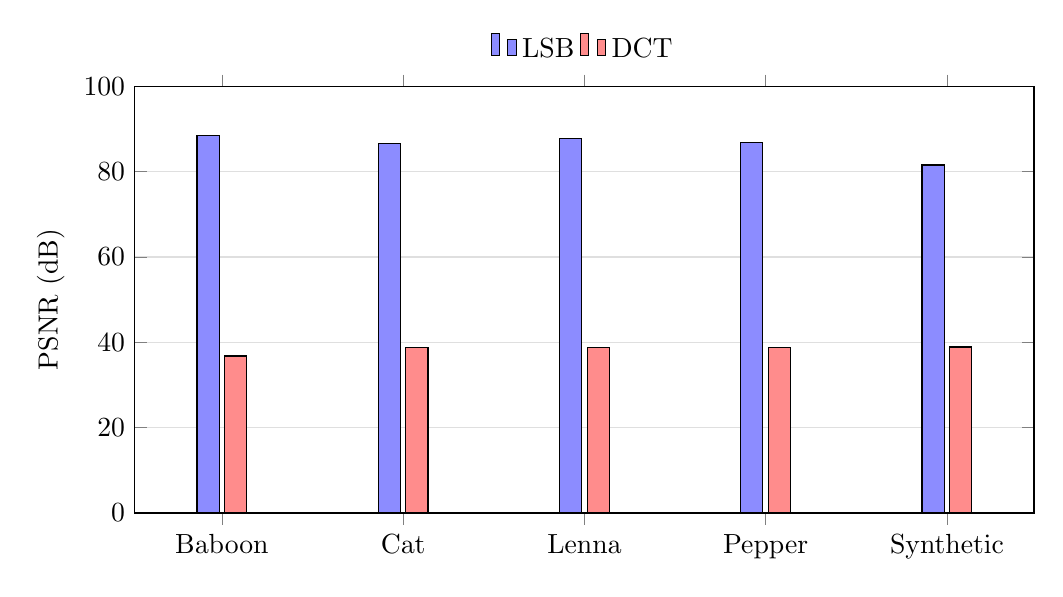
\begin{tikzpicture}
\begin{axis}[
  ybar, bar width=8pt,
  width=13cm, height=7cm,
  ylabel={PSNR (dB)},
  ymin=0, ymax=100,
  symbolic x coords={Baboon,Cat,Lenna,Pepper,Synthetic},
  xtick=data,
  legend style={at={(0.5,1.03)}, anchor=south, legend columns=2, draw=none},
  enlarge x limits=0.12,
  ymajorgrids=true, grid style={gray!25}
]
\addplot[fill=blue!45] coordinates
  {(Baboon,88.48) (Cat,86.52) (Lenna,87.69) (Pepper,86.81) (Synthetic,81.57)};
\addplot[fill=red!45] coordinates
  {(Baboon,36.80) (Cat,38.76) (Lenna,38.71) (Pepper,38.71) (Synthetic,38.91)};
\legend{LSB, DCT}
\end{axis}
\end{tikzpicture}
\end{document}
